\subsection{Future Works}\label{subsec:futureWorks}
This section explores potential features for TREAT, and research that relates to the use of the program, that are not implemented or performed at the time of release of this paper.

\subsubsection{Pruning}\label{futureWorks:pruning}
A paper by Daws et al. \cite{Daws1996} describes clock pruning in timed automata. There are several methods of pruning clocks, that are not part of TREAT at the time of writing this paper.
Clock pruning is one example of an area in which further optimization may be found. It should be noted, however, that adding several more pruning steps, might decrease performance in certain areas.
This conundrum should be adressed with testing and benchmarking, to determine which pruning algorithms would effectively improve performance in relevant areas.

A pruning method that was previously in development for TREAT, was "final state pruning", in which, final states would be merged together. This method was ultimately not implemented, because we were unable to formally define a proper algorithm, and therefore could not be certain that a pruned TA would always be equivalent to its un-pruned counterpart.
\cref{fig:finalStateBefore} shows a TA before it has been pruned using the proposed final state pruning method.
% Generated by: TimedRegex, Version = 1.0.0.0
% Date 5/23/2024 12:09:41 PM
\usetikzlibrary {automata,positioning}
% "A|BA"
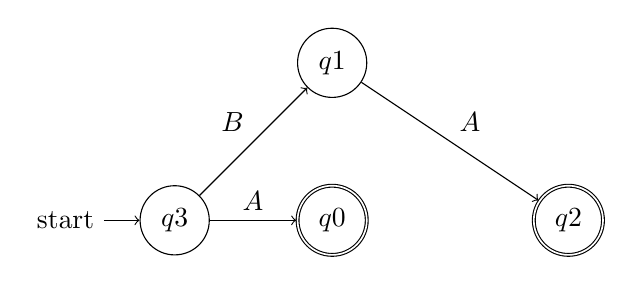
\begin{tikzpicture}[auto]
    \node[state, accepting] at (2, 0)(q0){$q0$};
    \node[state] at (2, 2)(q1){$q1$};
    \node[state, accepting] at (5, 0)(q2){$q2$};
    \node[state, initial] at (0, 0)(q3){$q3$};
    
    \path[->]
        (q1)edge node{$A$}(q2)
        (q3)edge node{$A$}(q0)
        (q3)edge node{$B$}(q1)
        ;
\end{tikzpicture}
\captionof{figure}{Before pruning with final state pruning}
\label[figure]{fig:finalStateBefore}



\cref{fig:finalStateAfter} shows what that same TA would look like after pruning. The two final states have been merged, while all edges one could take to reach the final state, remains the same as before pruning.

\usetikzlibrary {automata,positioning}
% "A|BA"
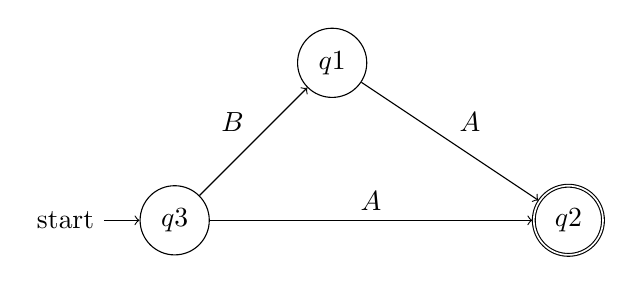
\begin{tikzpicture}[auto]
    \node[state, accepting] at (5, 0)(q2){$q2$};
    \node[state] at (2, 2)(q1){$q1$};
    \node[state, initial] at (0, 0)(q3){$q3$};
    
    \path[->]
        (q1)edge node{$A$}(q2)
        (q3)edge node{$A$}(q2)
        (q3)edge node{$B$}(q1)
        ;
\end{tikzpicture}
\captionof{figure}{After pruning with final state pruning}
\label[figure]{fig:finalStateAfter}


\subsubsection{TRE from TA}
According to Eugene et al.\cite{Eugene2001}, it should always be possible to create a TRE from a TA that is equivelant to the TA it was created based on.
A future TREAT project could use the methods described by Eugene et al., in order to create TREs from a given representation of a TA, such as one from a UPPAAL file.
This would involve parsing the UPPAAL file, converting that information into an automaton, and then converting that automaton to a TRE.
While this feature was not prioritized for implementation in the version of TREAT accompanying the release of this paper, the feature may prove useful for representing TAs as TREs, and even converting a TA originally represented in one format, such as UPPAAL, to a different one, such as TikZ.

